\chapter{Le modifiche al SIMIOR}
Per accomodare le nuove funzionalità è stato necessario fare delle modifiche strutturali al SIMIOR, spaziando dal database a classi di gestione dei dati interne al front-end del progetto.
\section{Modifiche strutturali}
Le modifiche fatte si possono raggruppare in tre punti:
\begin{itemize}
	\item Database
	\item Archivio Statico
	\item Front-End
\end{itemize}
Oltre al database che contiene i dati creati dagli utenti, il SIMIOR possiede dei dati "statici" che raramente richiedono una modifica, un esempio di questi dati sono i codici degli antibiotici definiti dal sistema ATC/DDD (Anatomical Therapeutic Chemical/Defined Daily Dose) o i codici dei microorganismi definiti dall'Istituto Superiore di Sanità.
Quando viene effettuato un inserimento di un antibiogramma (sia tramite la nuova funzionalità sia manualmente) il sistema effettua una ricerca in questo archivio statico per estrarre il codice relativo al microrganismo/antibiotico, ma inizialmente questi nomi erano in lingua inglese (sempre seguendo il sistema di origine dei dati) causando il fallimento dell'estrazione. Per ovviare a questo problema si è prima provveduto ad aggiornare l'archivio con la versione italiana e in secondo luogo aggiungendo la possibilità di avere un valore alternativo per casi particolari verificati in alcuni referti.
Che altro ho cambiato?
\newpage
\section{Implementazione FrontEnd}
L'utente può utilizzare la funzionalità recandosi nella sezione \textit{infezione, contaminazione o colonizzazione} di un qualsiasi ricovero, dove troverà una scheda contenente l'essenziale per poter allegare un referto e procedere con il caricamento.
\subsection{Localizzazione della funzionalità}
\begin{figure}[h!]
	\centering
	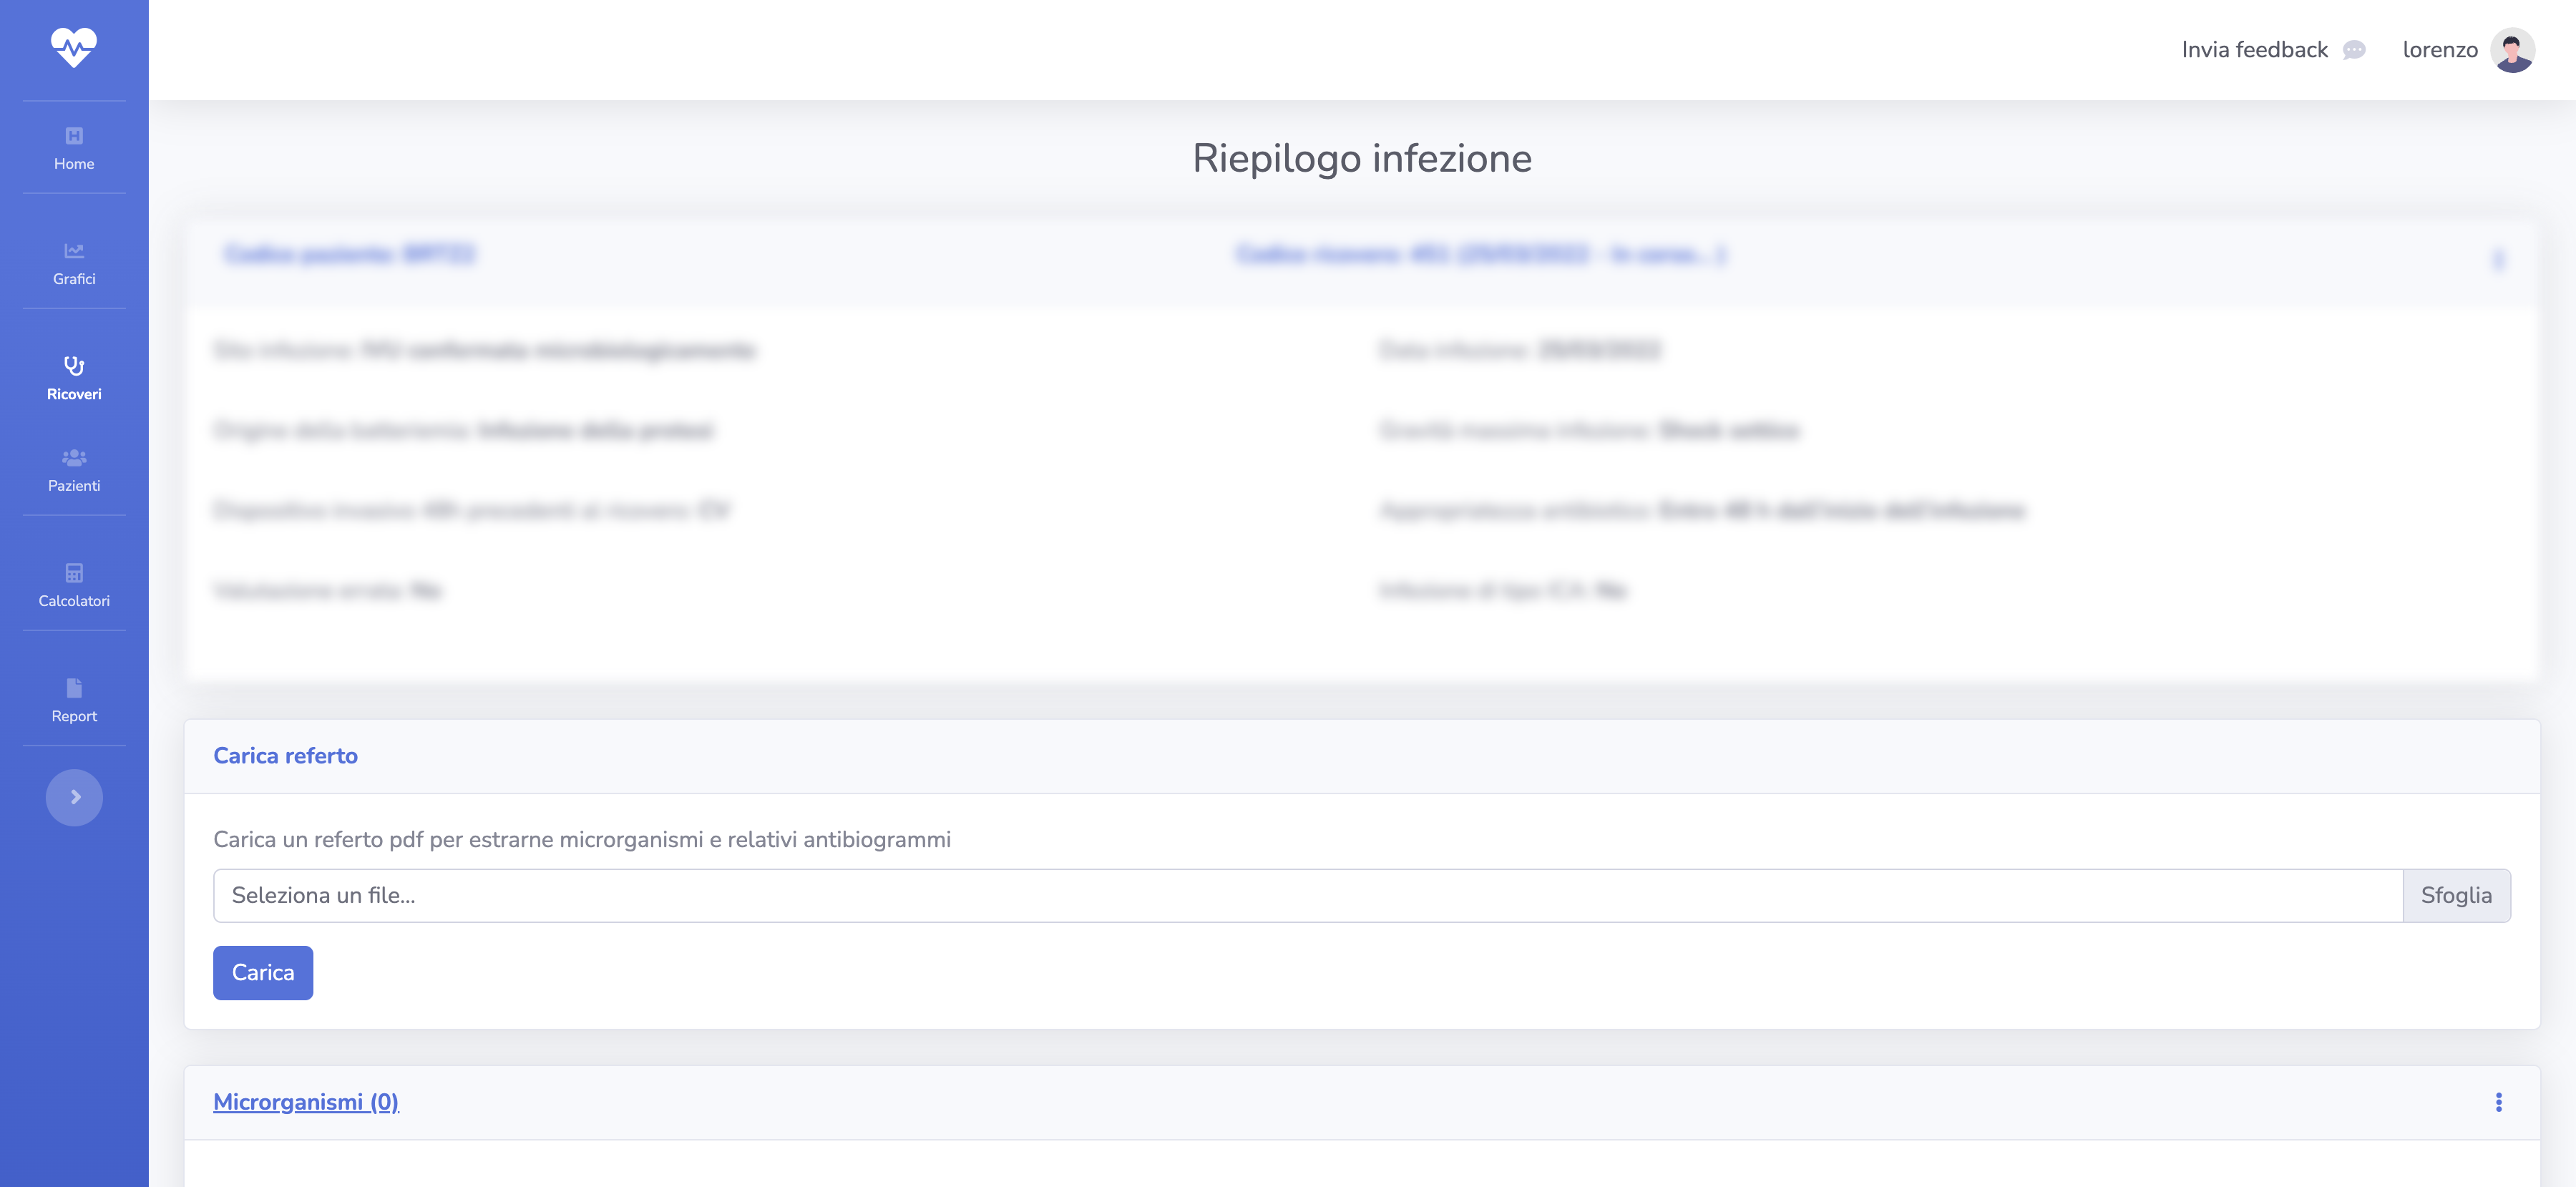
\includegraphics[width=.99\columnwidth]{images/feature_location.png}
	\caption{\textit{Scheda upload documento}}
	\label{fig:feature_location}
\end{figure}

La pressione del tasto \textit{"Sfoglia"} aprirà una schermata di dialogo gestita dal sistema che permetterà di selezionare il file determinato. Fatto questo l'utente procede alla pressione del tasto \textit{Carica} che lo porterà a una seconda pagina dove verranno mostrati i risultati dell'estrazione.
\subsection{La schermata dei risultati}

\begin{figure}[h!]
	\centering
	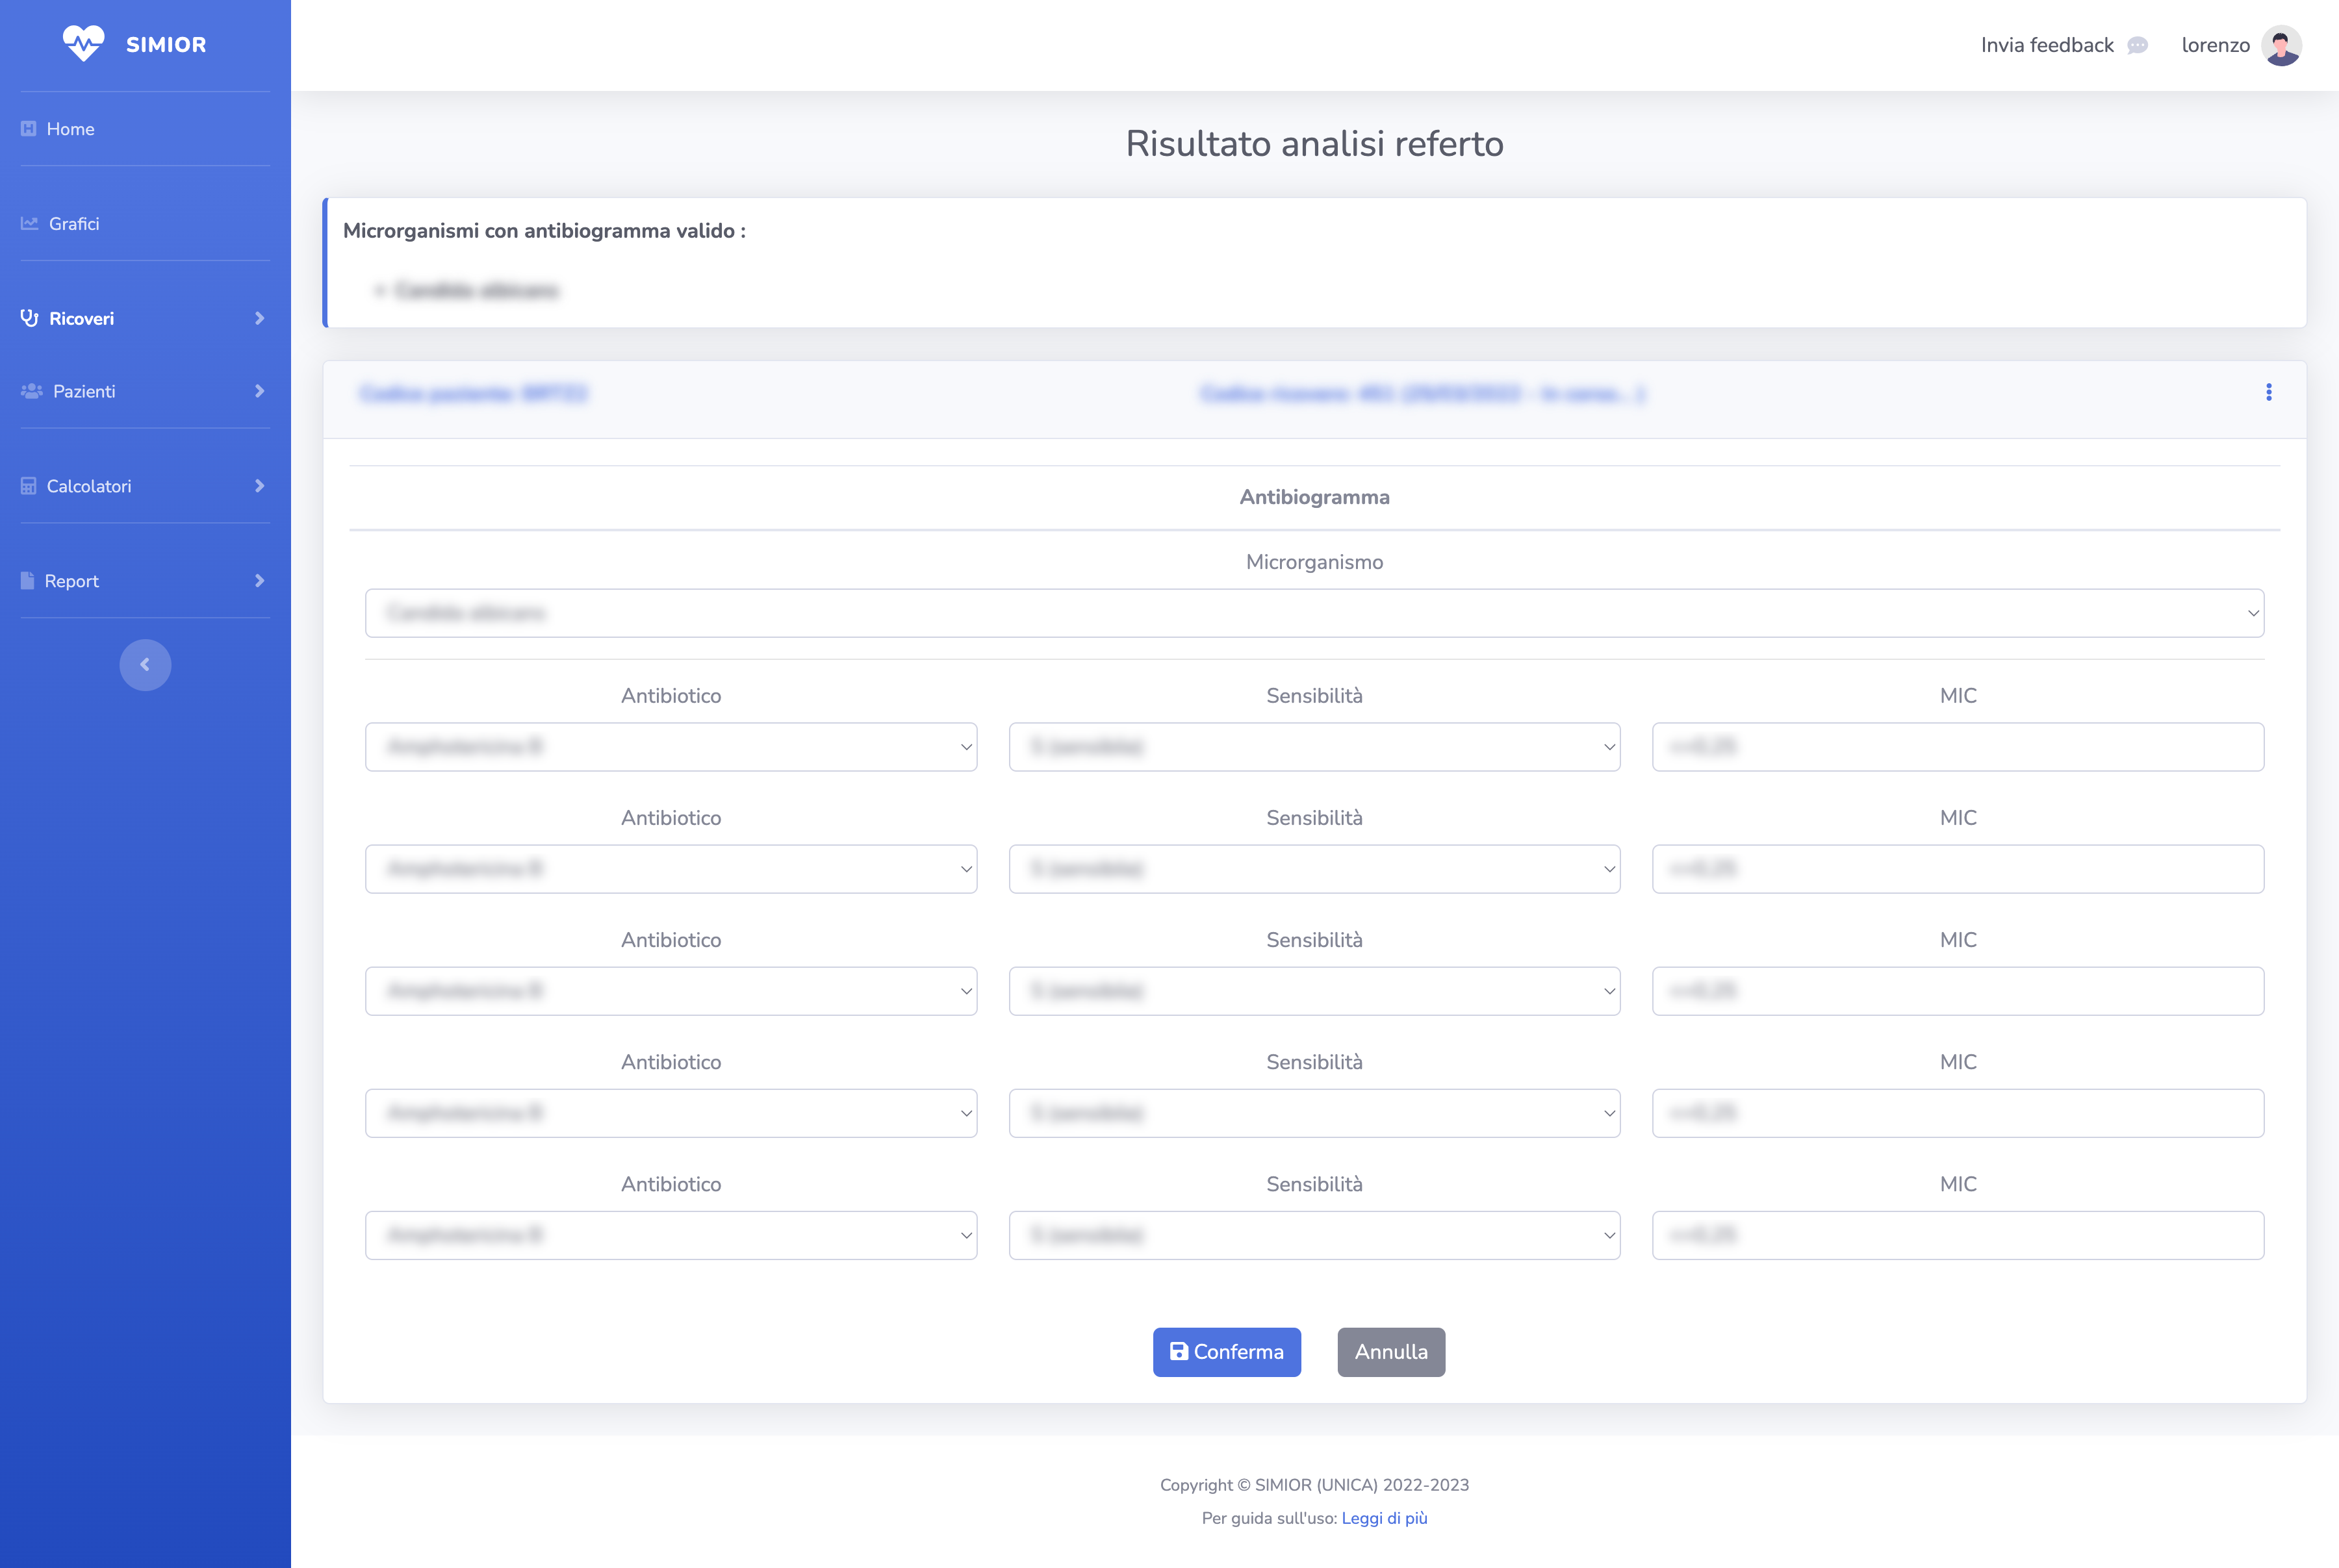
\includegraphics[width=.99\columnwidth]{images/extraction_result.png}
	\caption{\textit{Risultati estrazione}}
	\label{fig:extraction_result}
\end{figure}

\begin{figure}[h!]
	\centering
	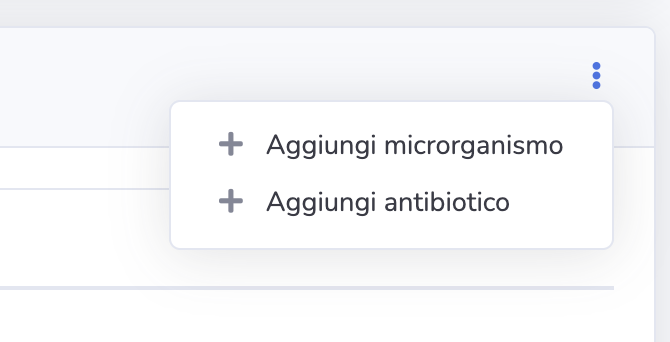
\includegraphics[width=.99\columnwidth]{images/new_object.png}
	\caption{\textit{Drop-down con le opzioni}}
	\label{fig:new_object}
\end{figure}